\section{Sequence Diagram}
\label{appendix:sequence_diagram}

% Anexo primero.

\begin{figure}[H]
    % cd plantuml && plantuml -tsvg sequence.txt && inkscape sequence.svg --export-filename=sequence.pdf && cd ..
    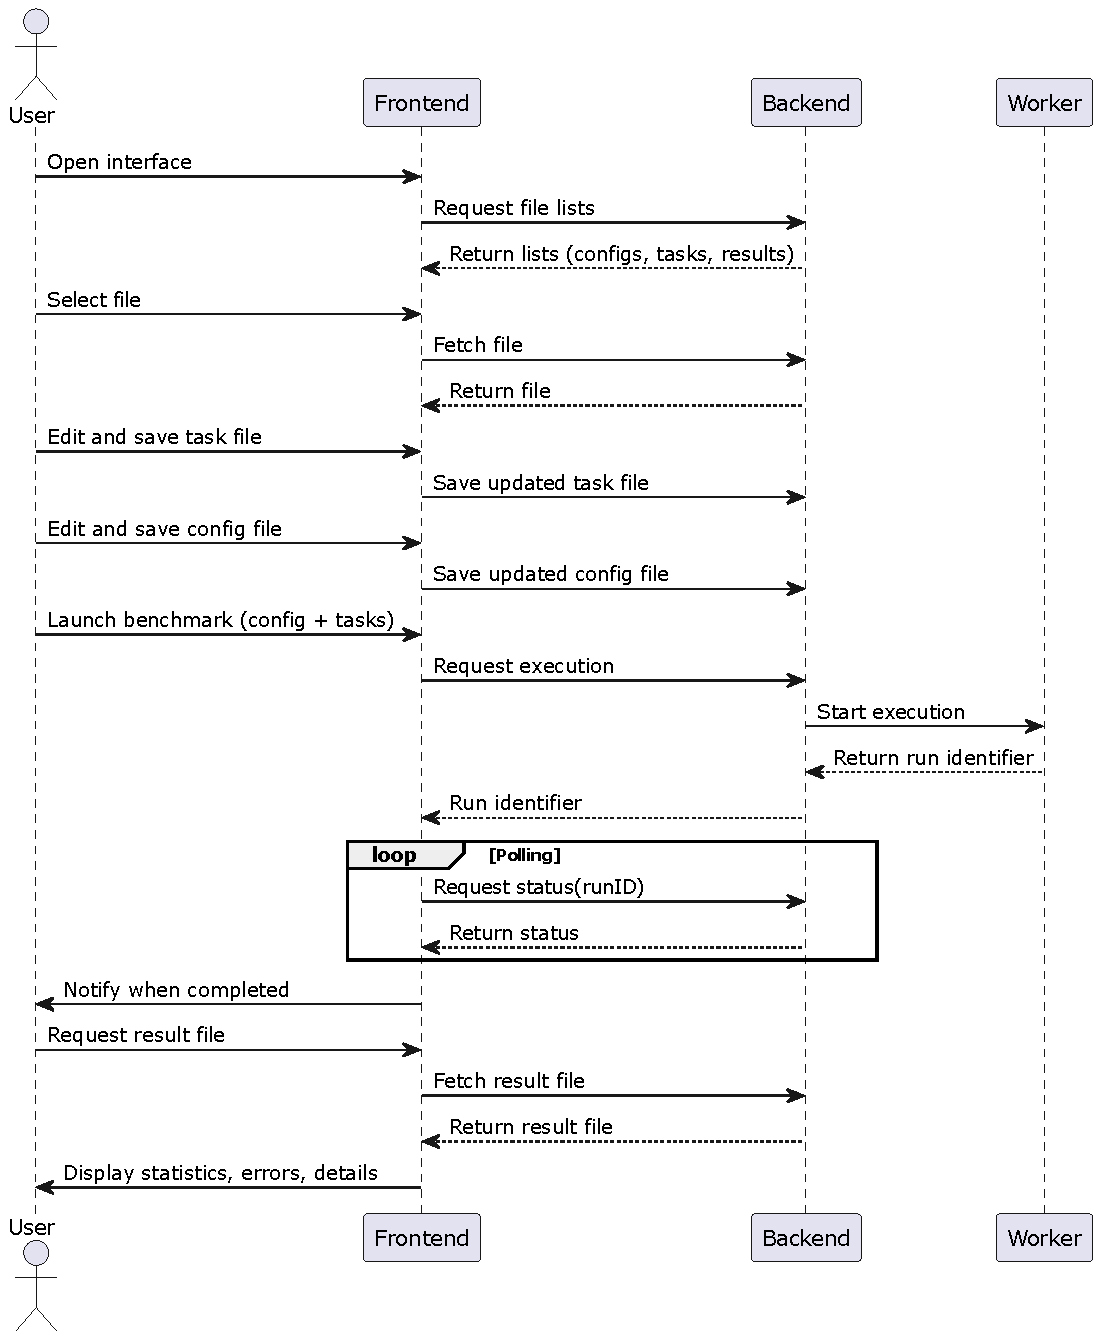
\includegraphics[width=0.9\textwidth]{./plantuml/sequence.pdf}
    \caption{Sequence Diagram.}
    \label{appendix:sequence}
\end{figure}

\section{User Interface Screenshots}
\label{appendix:ui_screenshots}

\begin{figure}[H]
    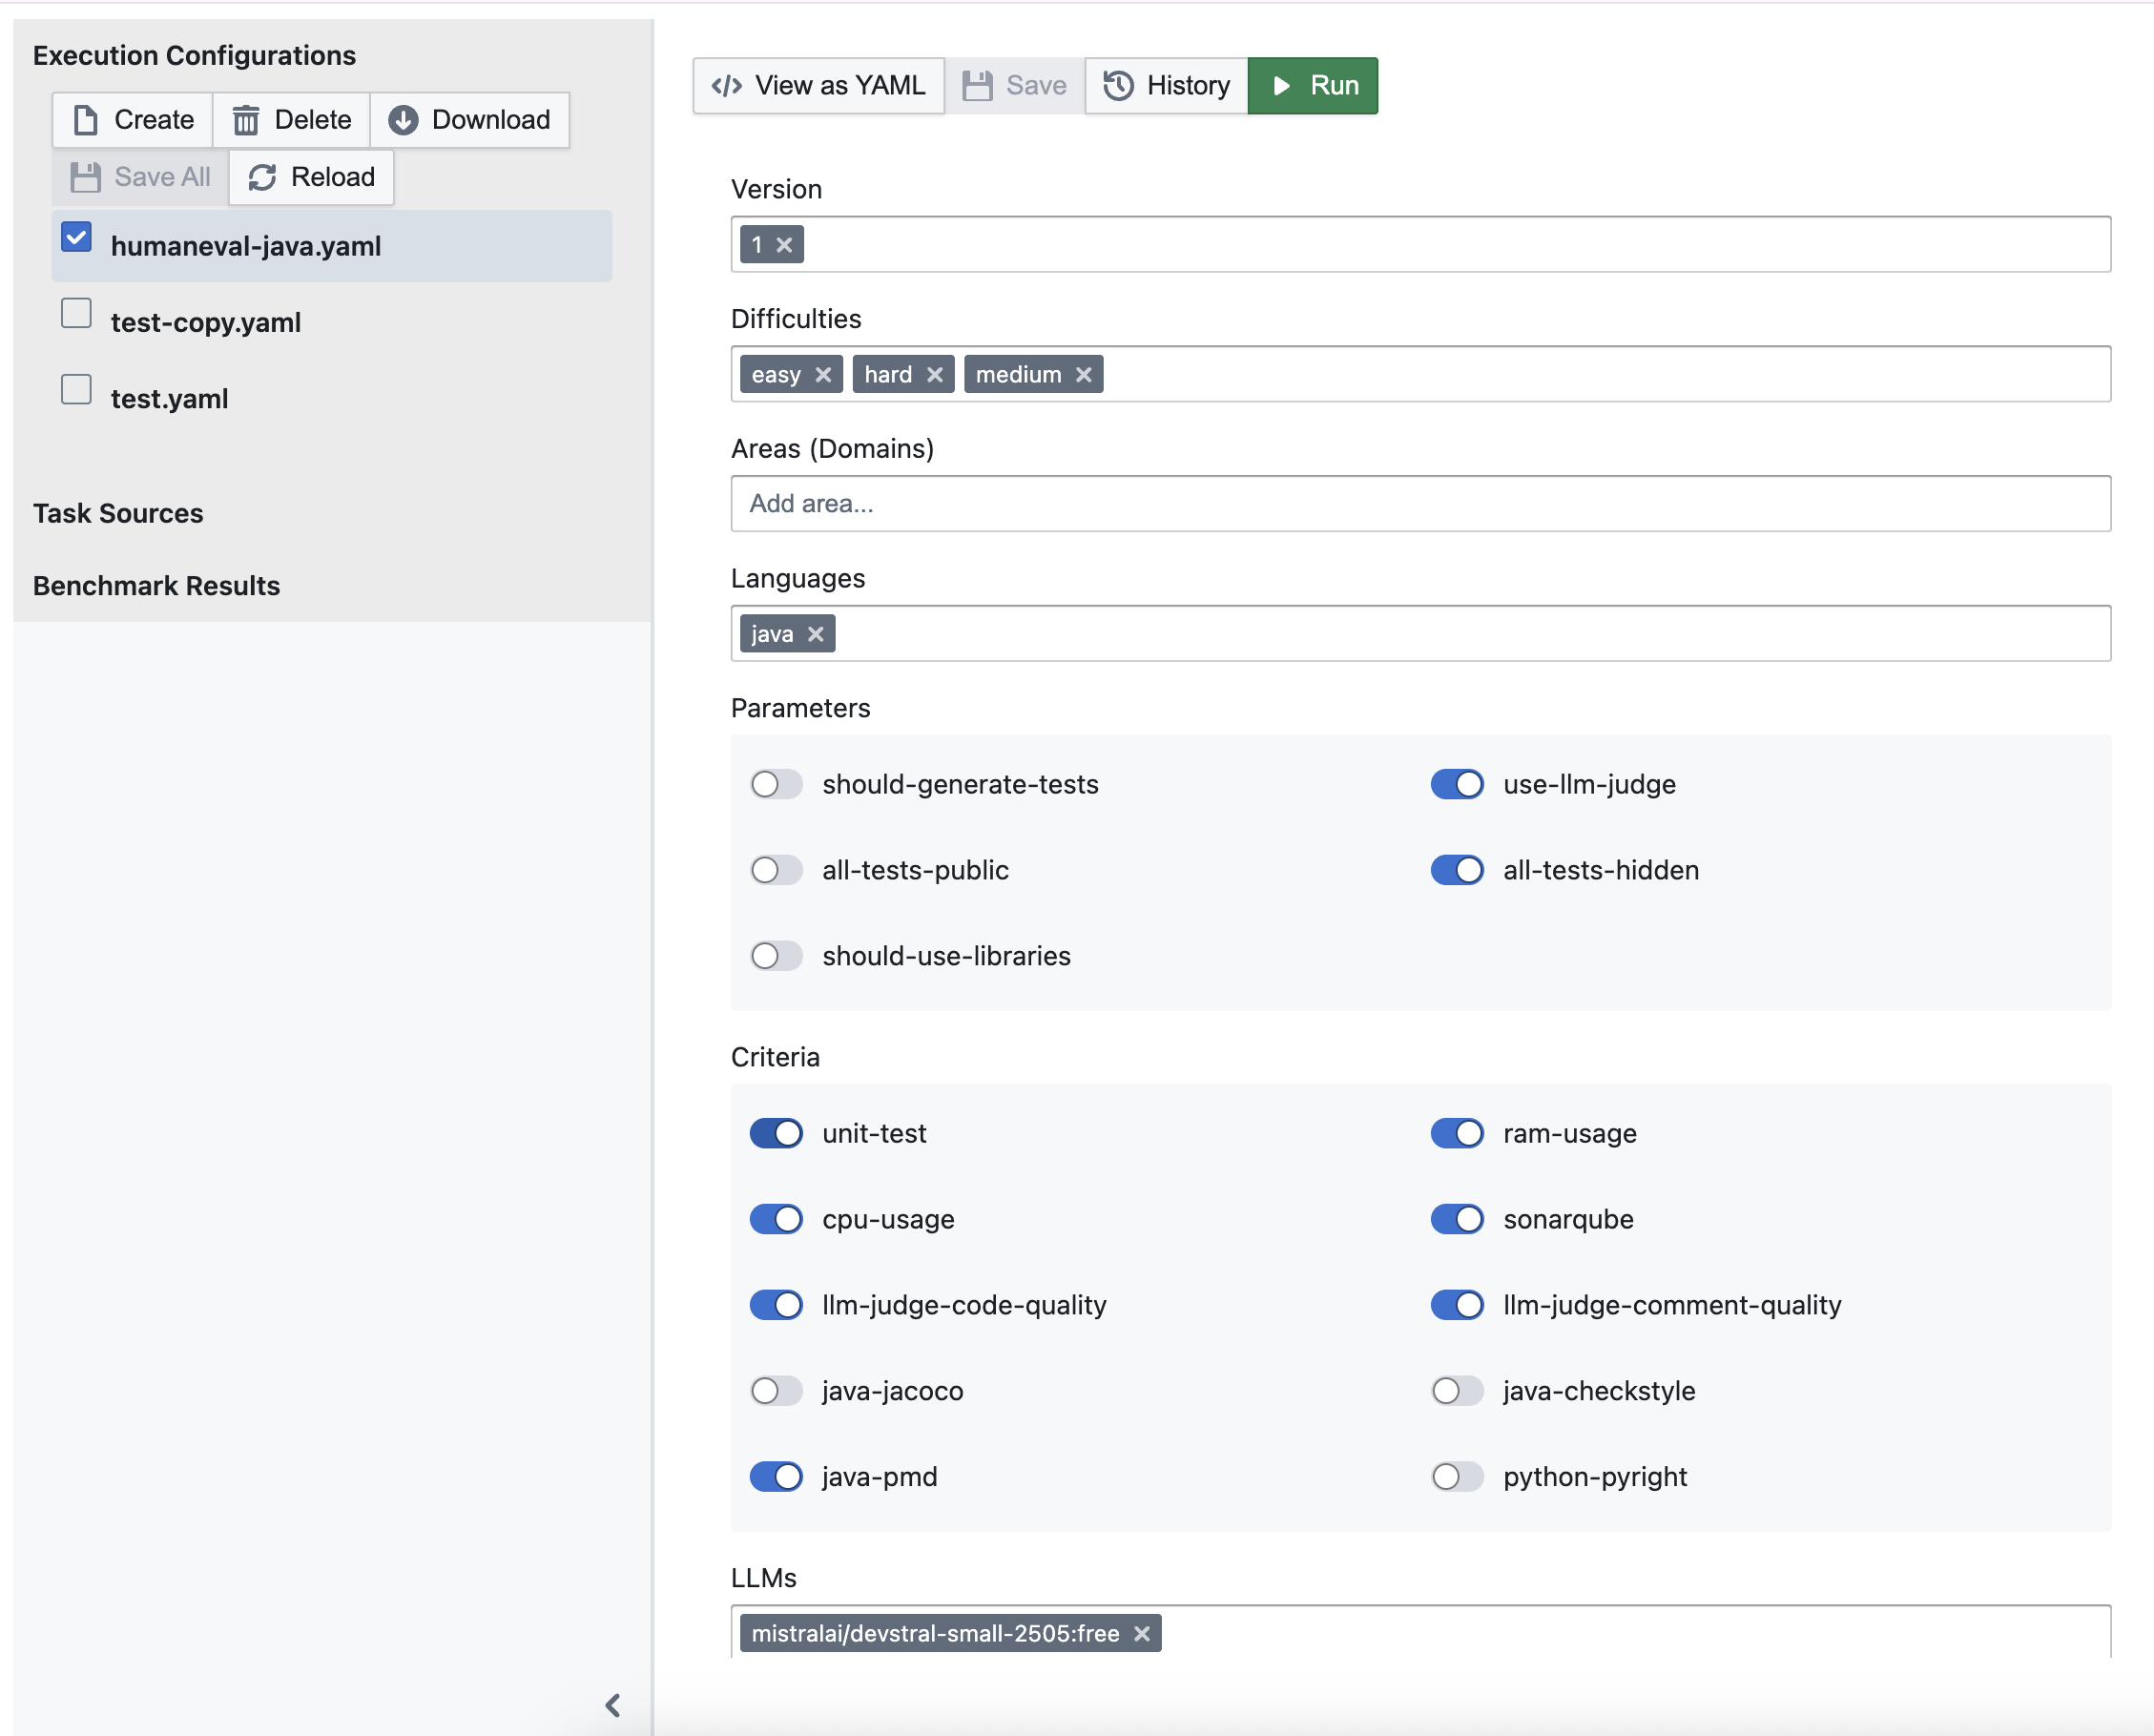
\includegraphics[width=0.9\textwidth]{./images/ui_exec_config}
    \caption{Execution Configuration visual editor.}
    \label{appendix:ui_exec_config}
\end{figure}


\begin{figure}[H]
    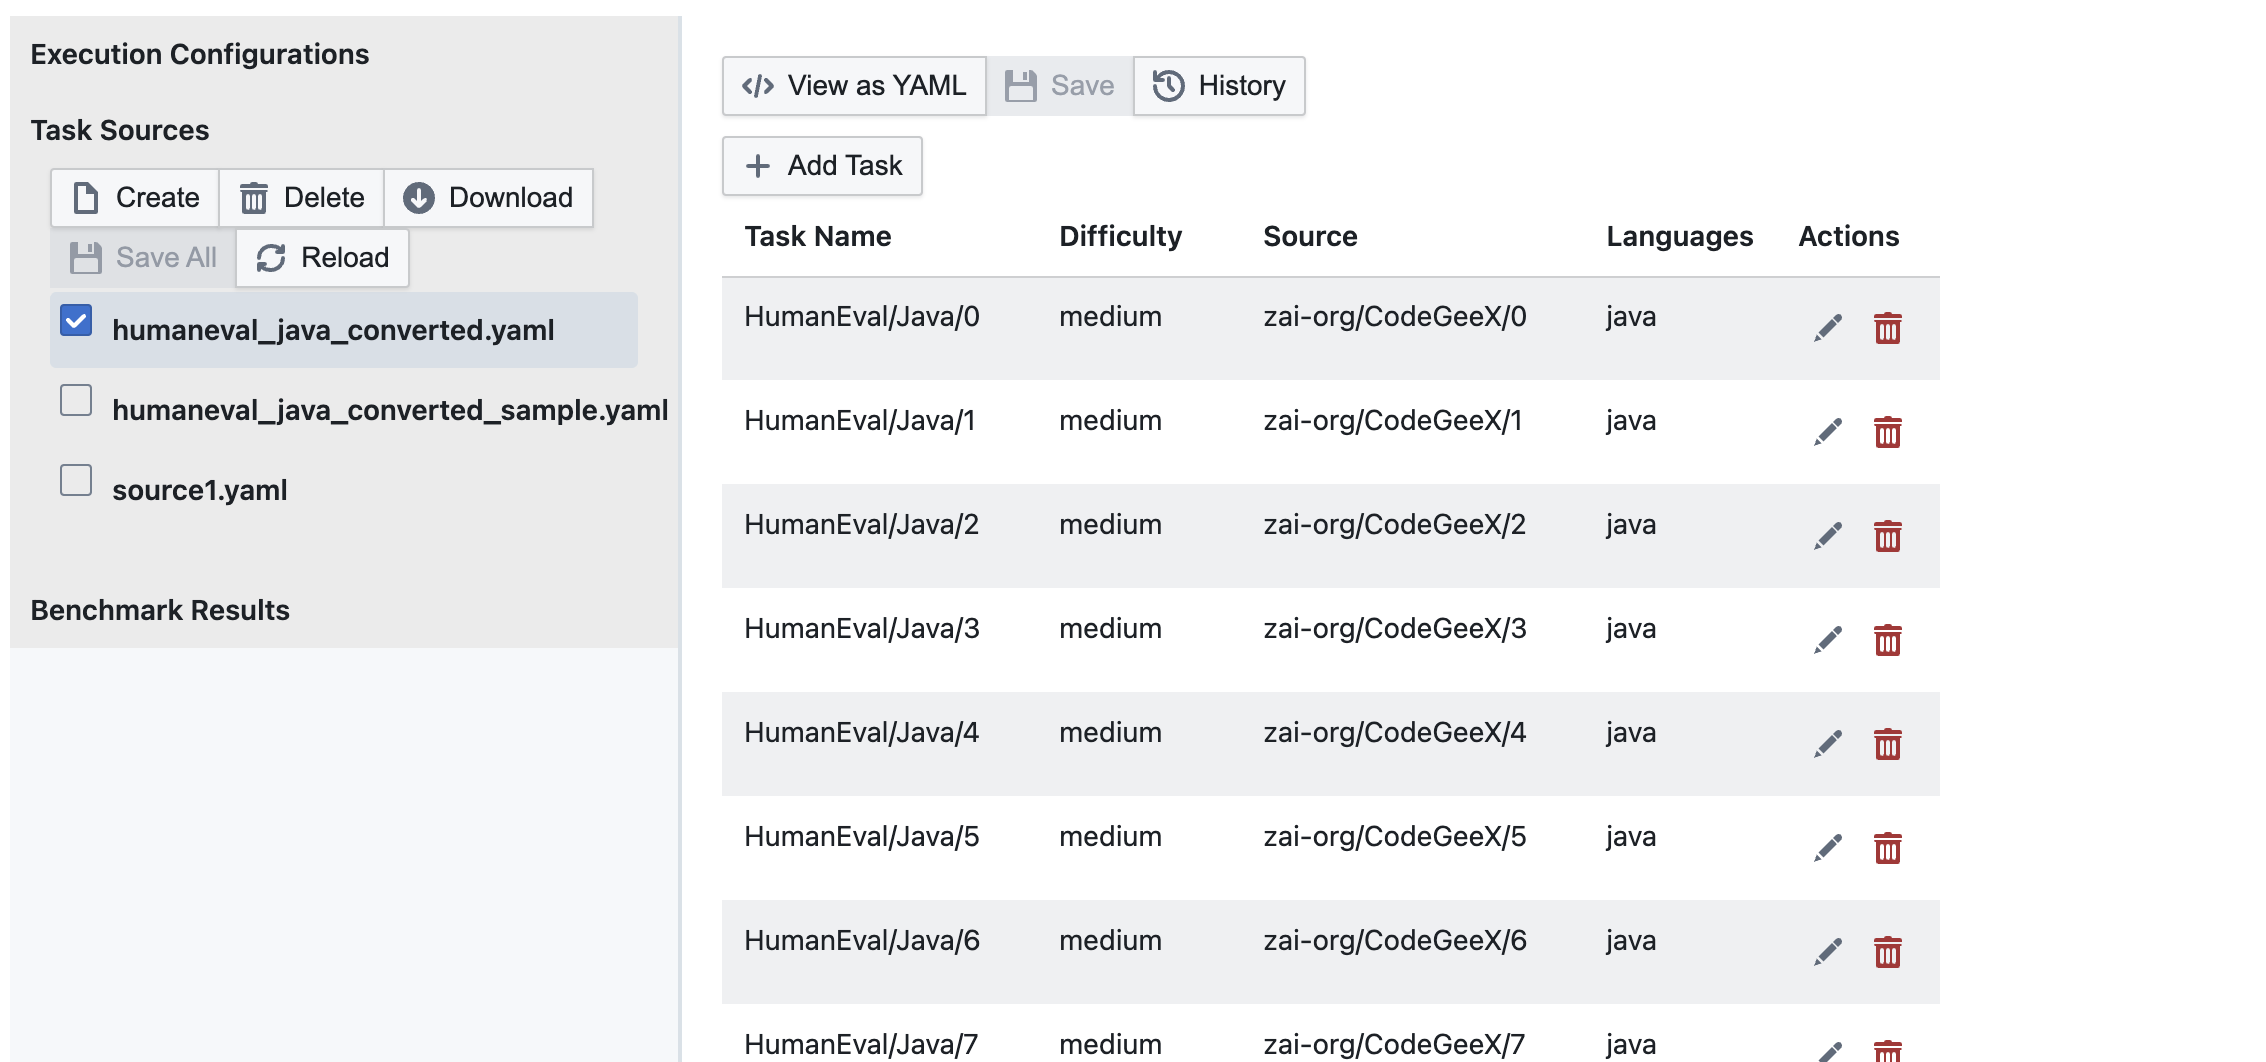
\includegraphics[width=0.9\textwidth]{./images/ui_task_source_list}
    \caption{Task Source visual editor. List of tasks in a Task Source.}
    \label{appendix:ui_task_source_list}
\end{figure}

\begin{figure}[H]
    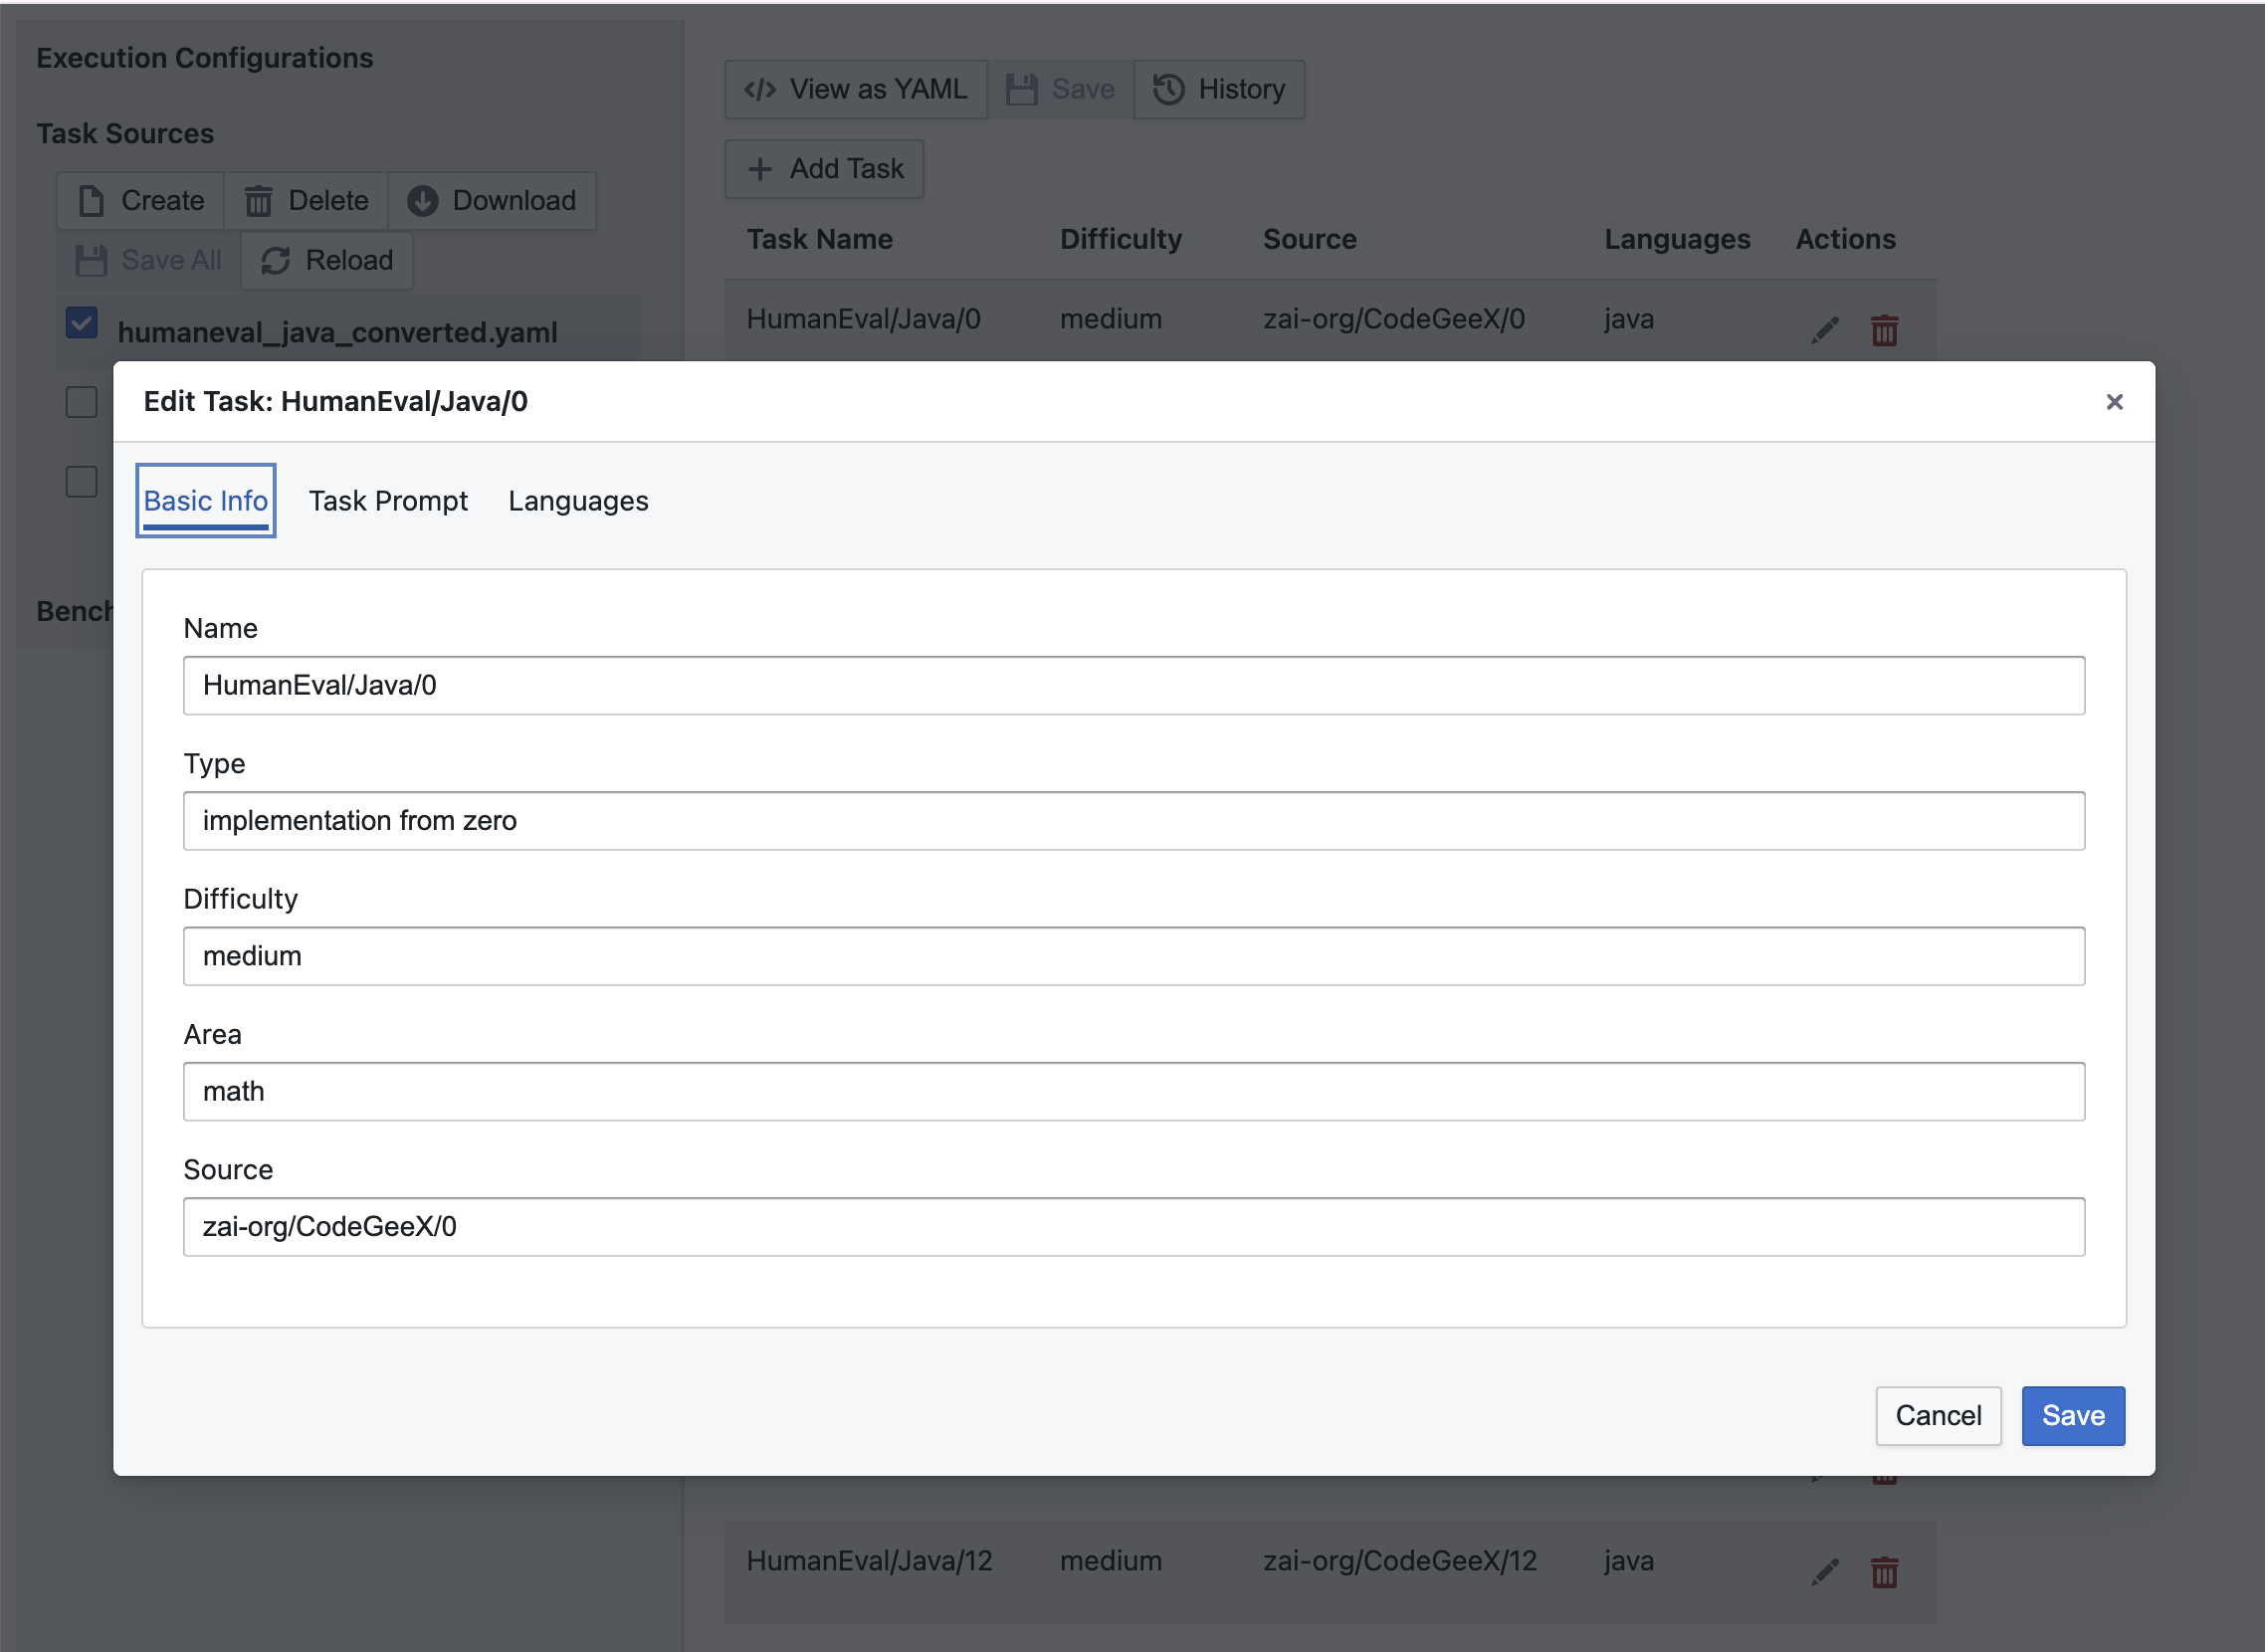
\includegraphics[width=0.9\textwidth]{./images/ui_task_source_info}
    \caption{Task Source visual editor. Basic information of a task.}
    \label{appendix:ui_task_source_info}
\end{figure}

\begin{figure}[H]
    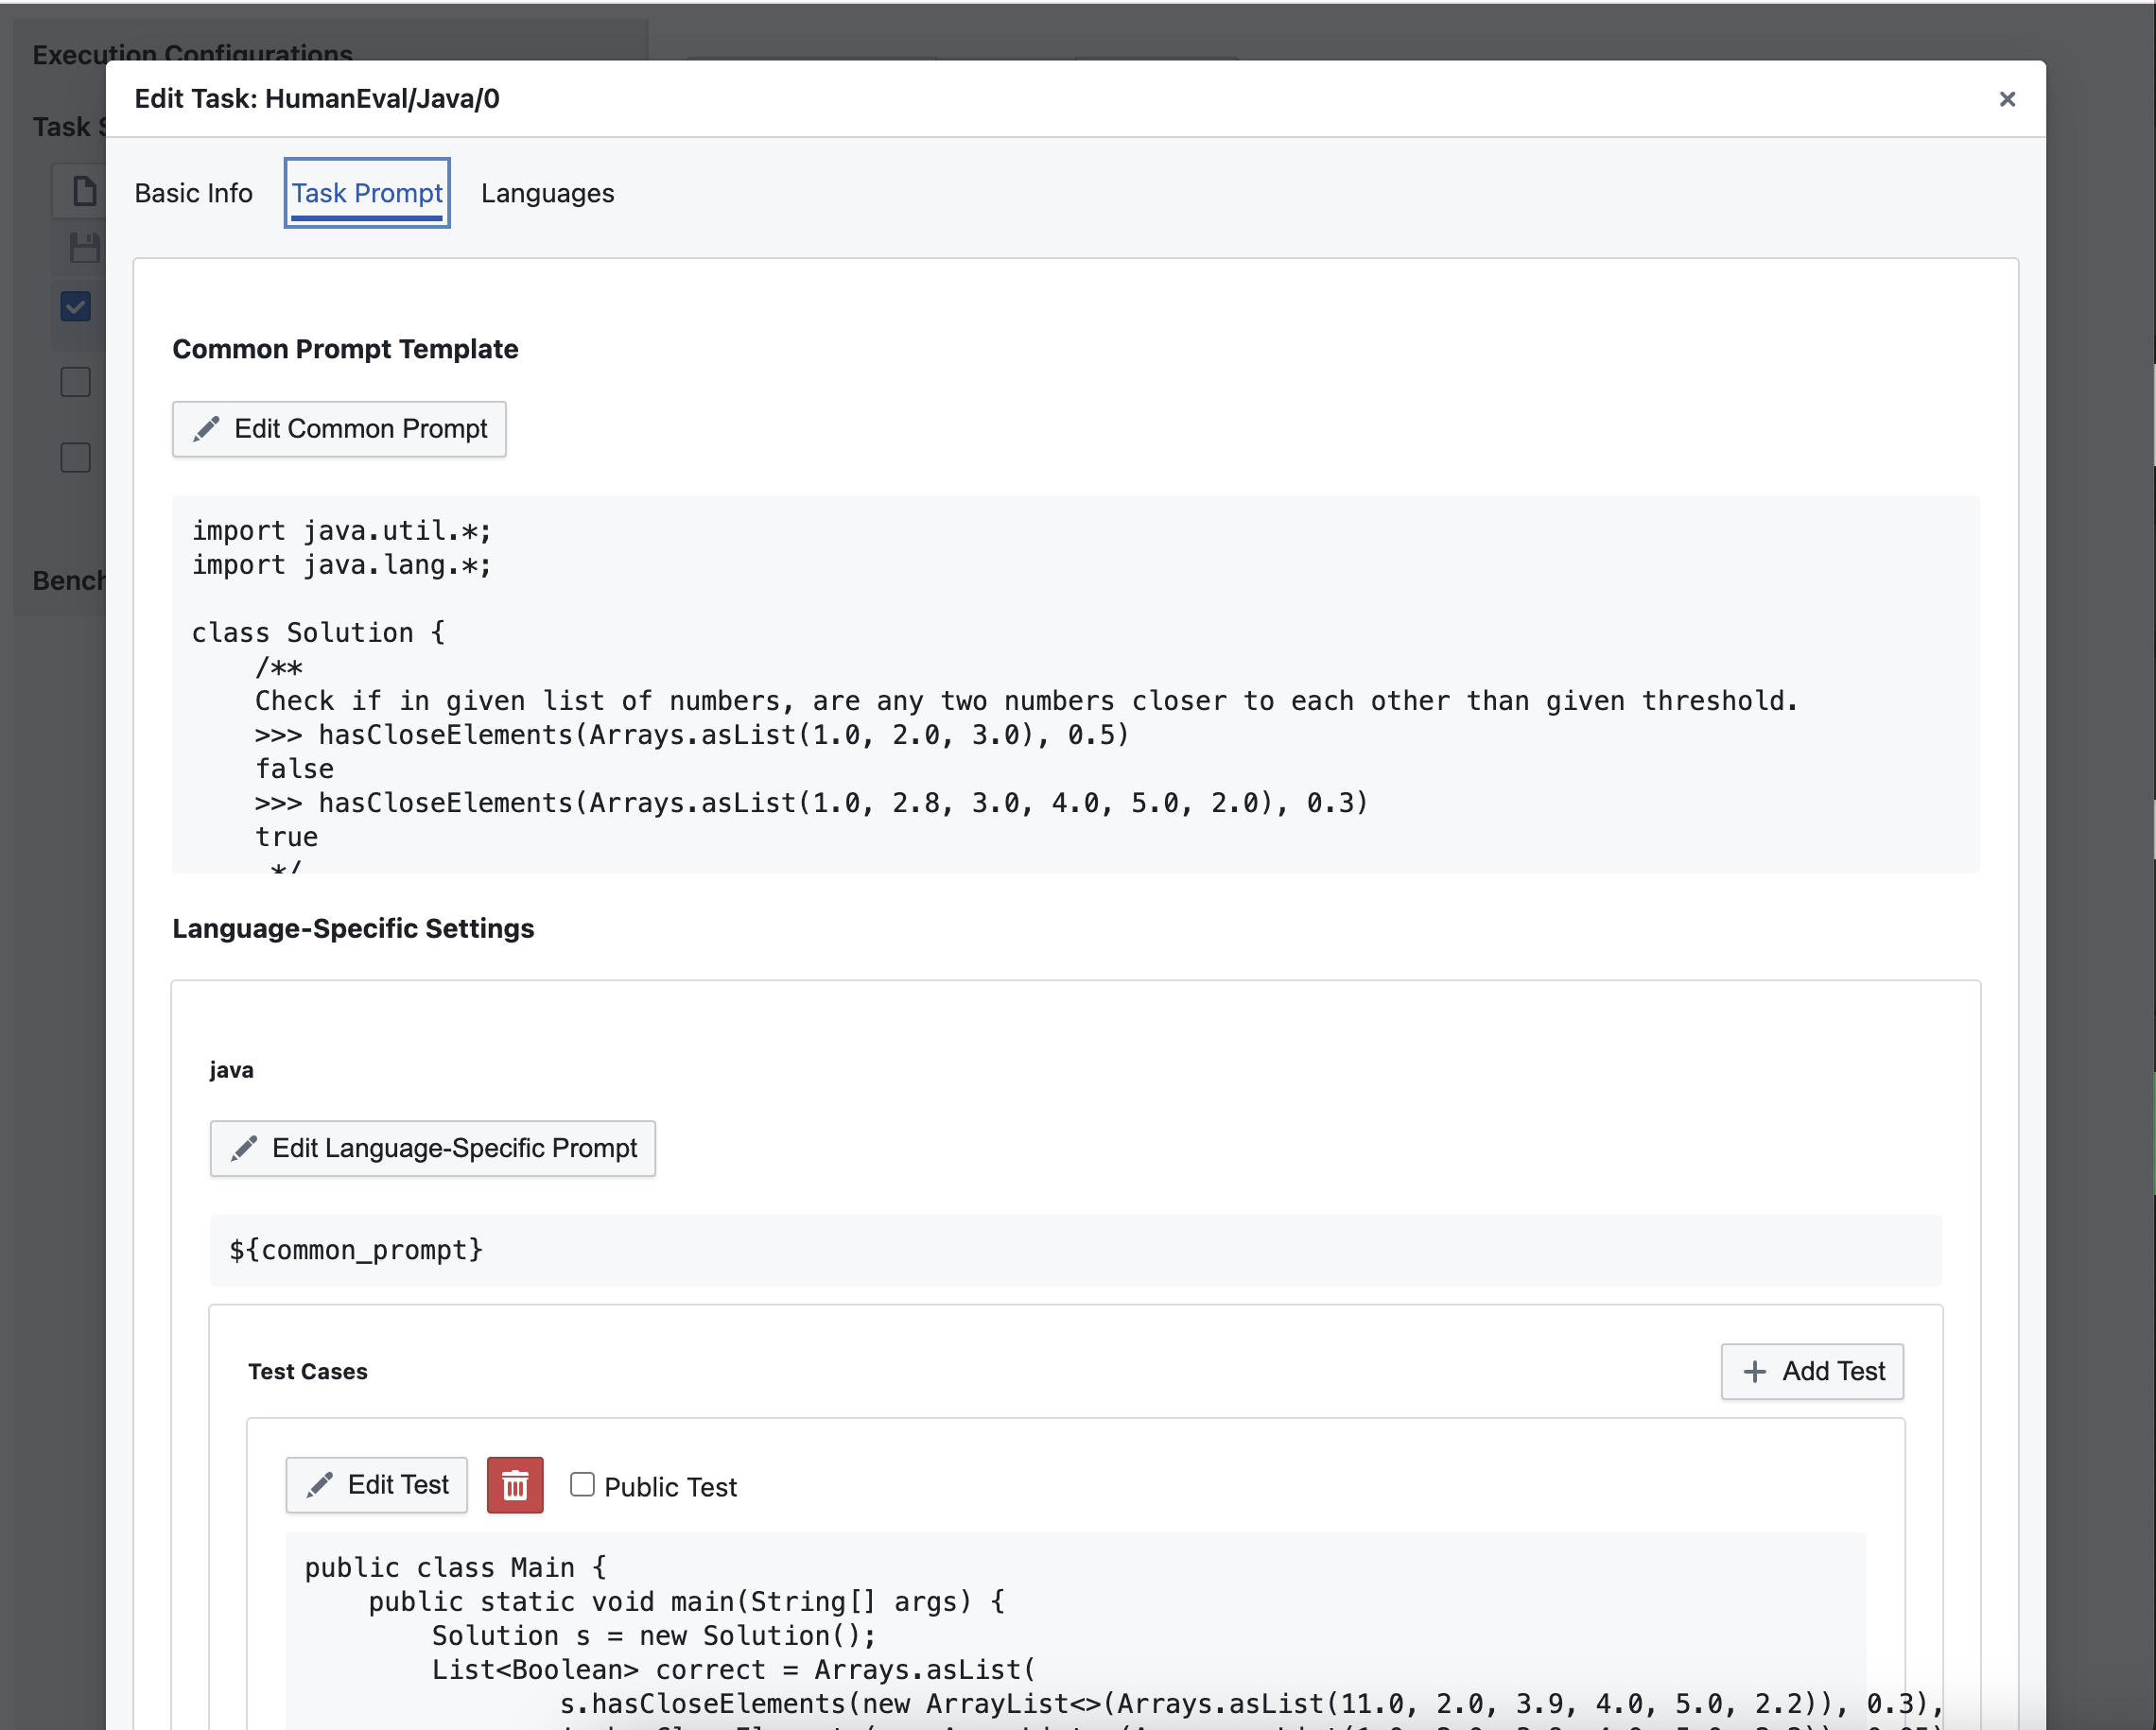
\includegraphics[width=0.9\textwidth]{./images/ui_task_source_prompts}
    \caption{Task Source visual editor. Prompts and tests of a task.}
    \label{appendix:ui_task_source_prompts}
\end{figure}

\begin{figure}[H]
    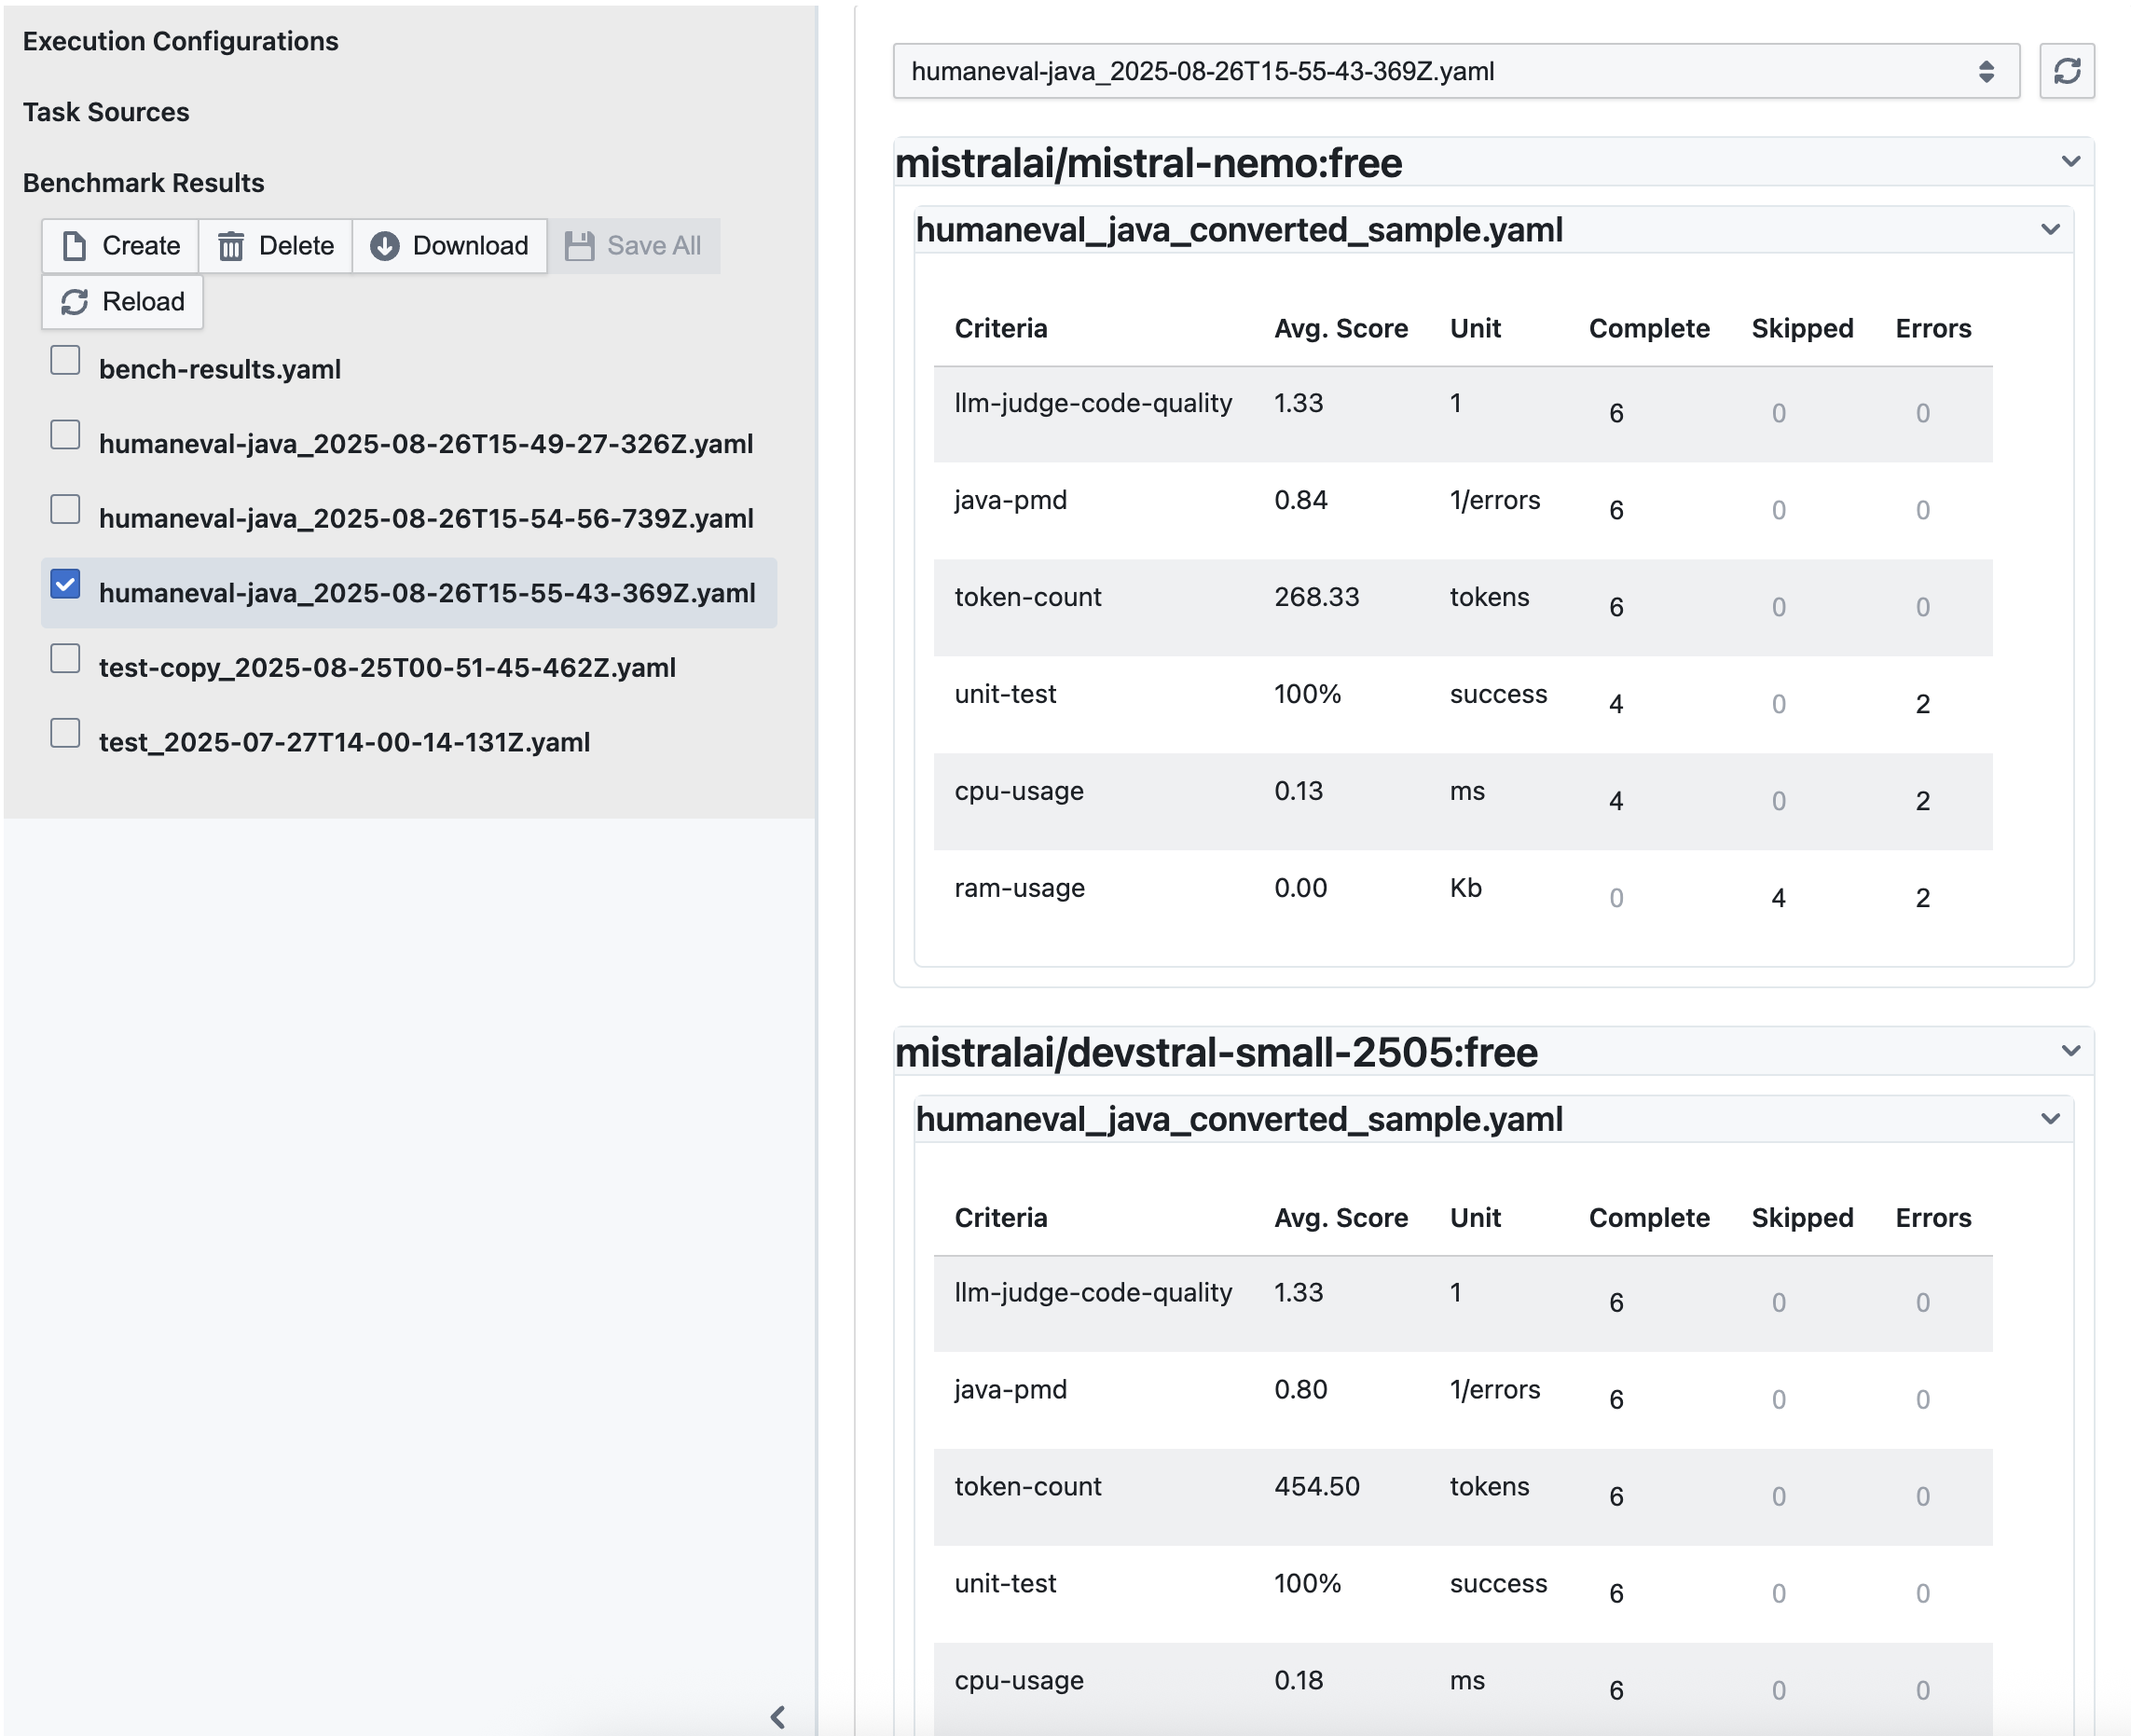
\includegraphics[width=0.9\textwidth]{./images/ui_results_multiple}
    \caption{Benchmark Results browser. }
    \label{appendix:ui_results_multiple}
\end{figure}

\begin{figure}[H]
    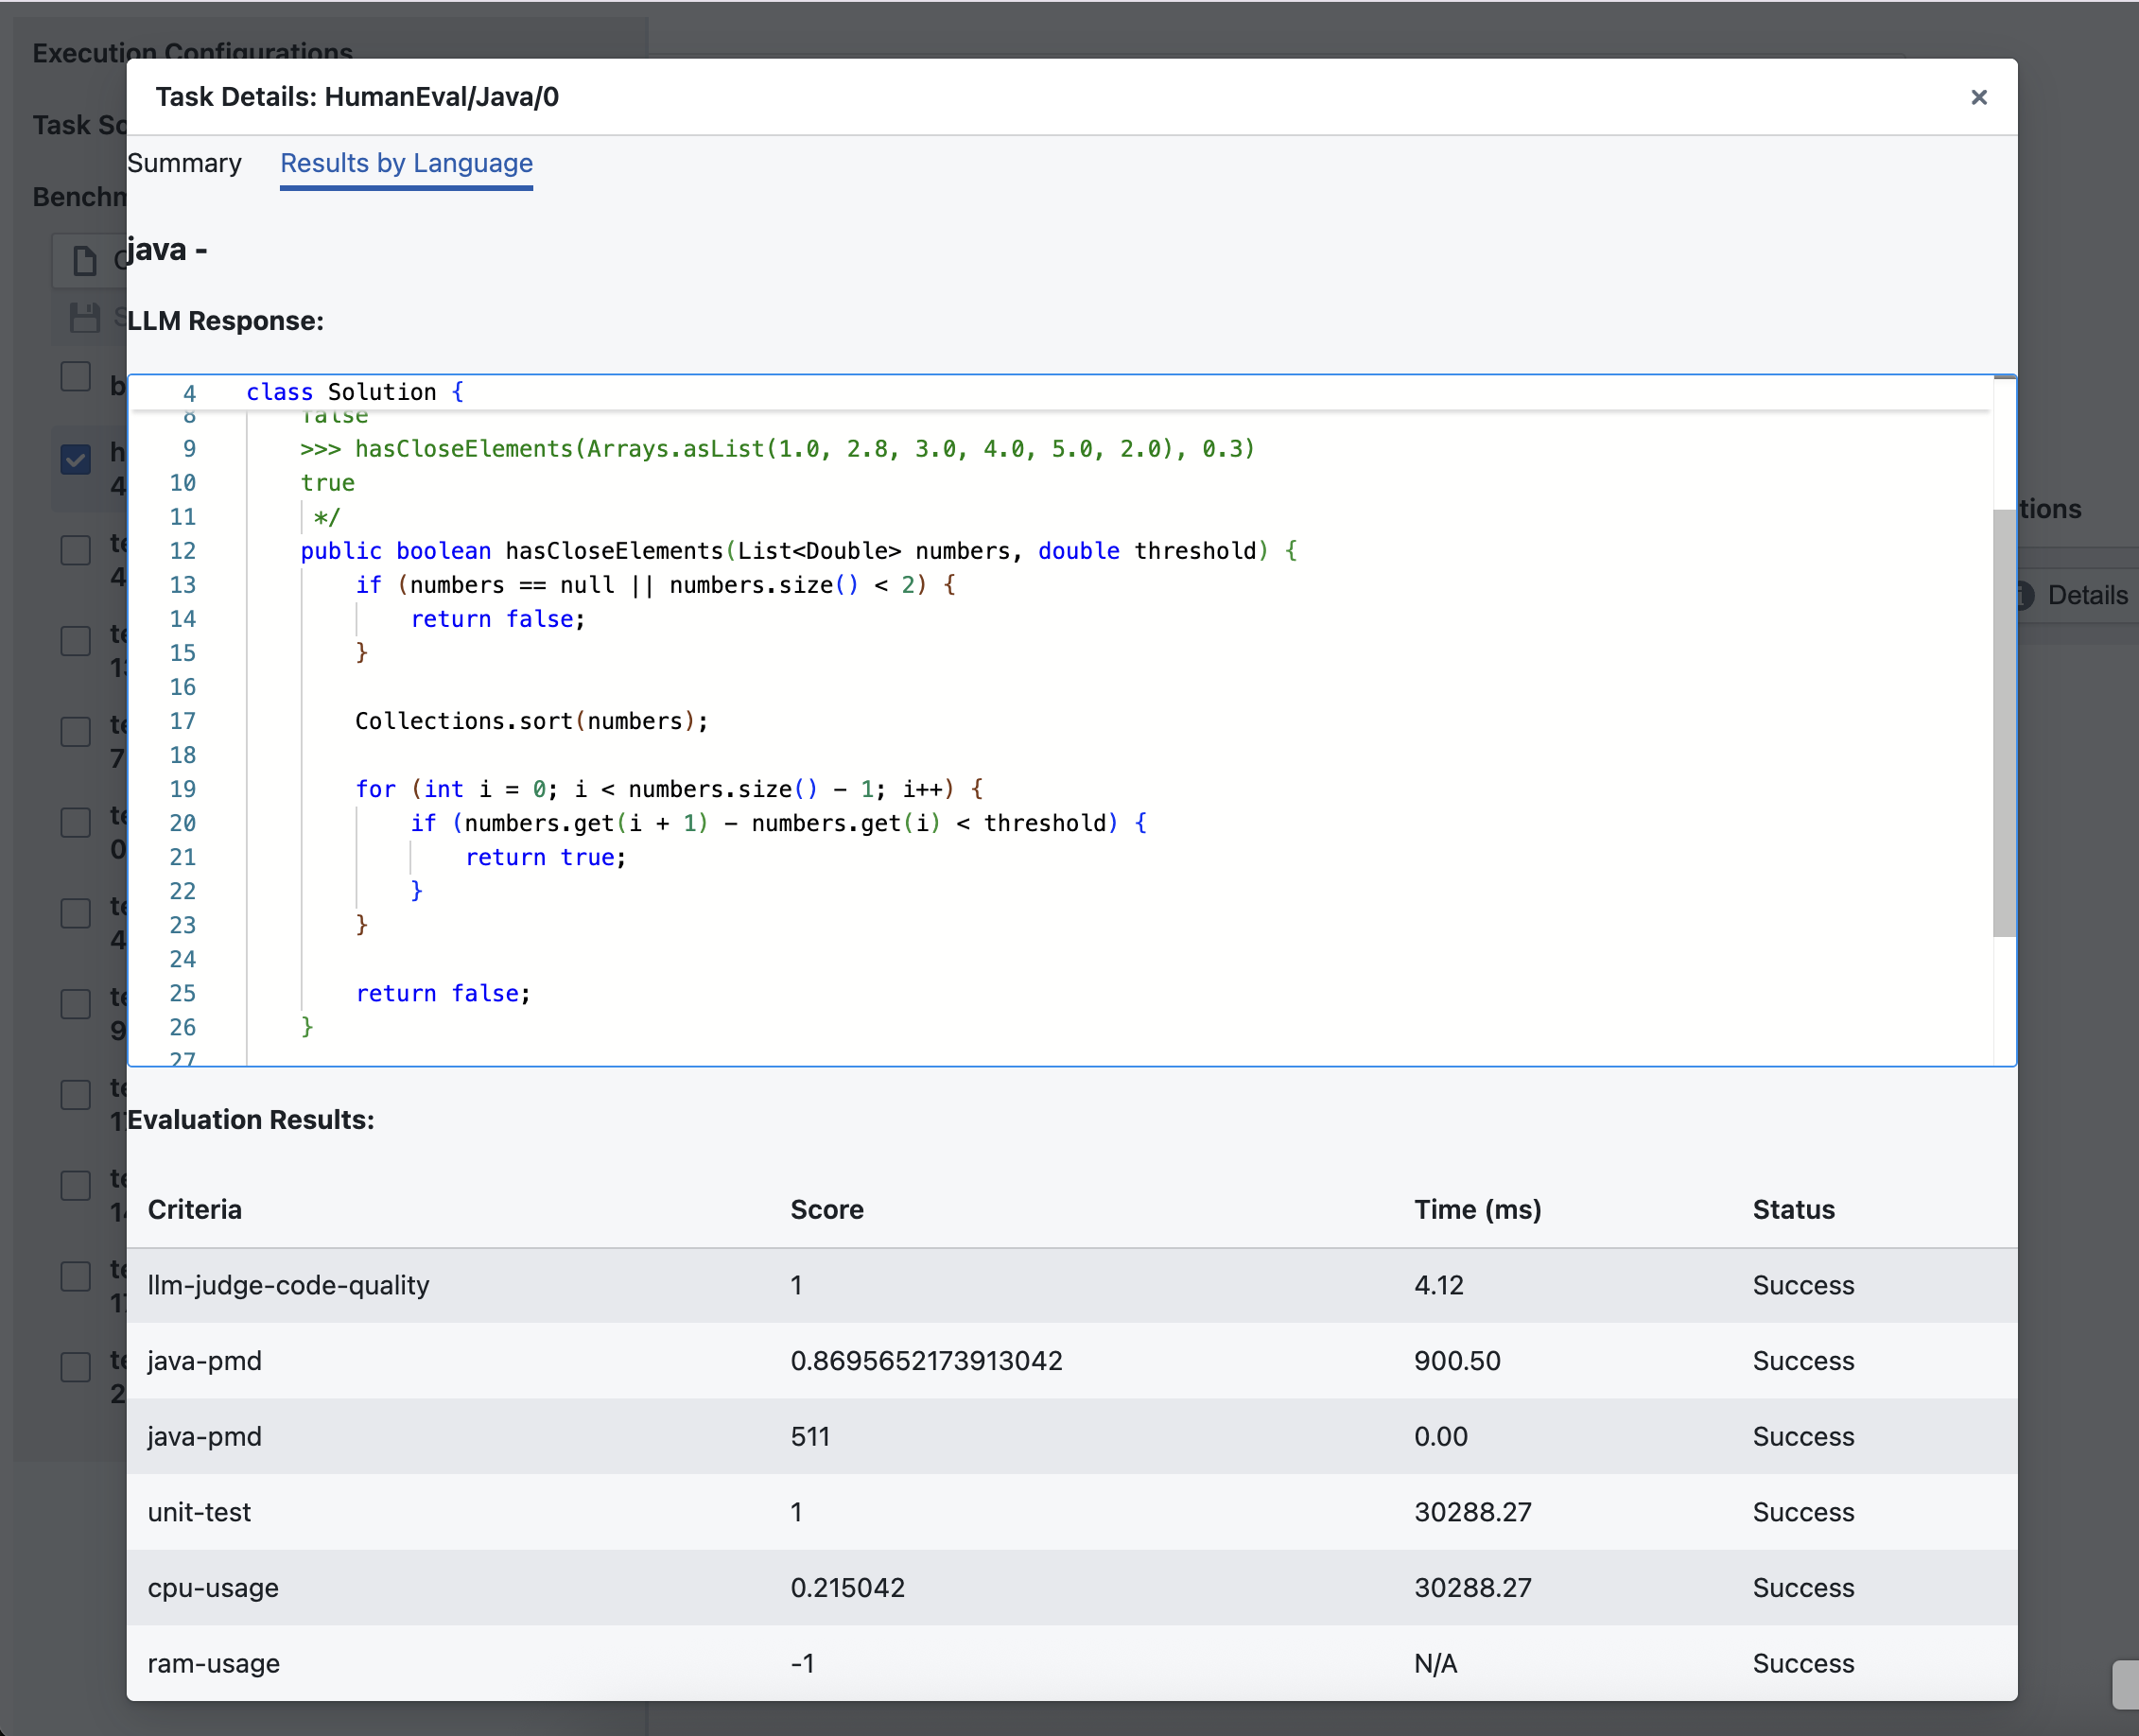
\includegraphics[width=0.9\textwidth]{./images/ui_result_single_task}
    \caption{Benchmark Results browser. }
    \label{appendix:ui_result_single_task}
\end{figure}

\section{Configuration and Result YAML Files}
\label{appendix:config_files}

\subsection*{Example of Configuration YAML file.}
\label{appendix:exec-config-example}
\codefileheader{exec-config-example-1.yaml}
\begin{minted}[linenos,breaklines,fontsize=\small]{yaml}
version: 1.0
difficulties:
  - easy
  - medium
  - hard
areas:
languages:
  - java
parameters:
  - name: should-generate-tests # if the LLM should generate tests for the code
    enabled: false
  - name: use-llm-judge         # if we want to check the results with an LLM-judge
    enabled: true
  - name: all-tests-public      # to include tests into a prompt as a reference
    enabled: false
  - name: all-tests-hidden      # if we don't want to give any tests as a reference
    enabled: true
criteria: # list of criteria to evaluate the solutions
  - name: unit-test         # only for languages that we can run in a sandbox
    enabled: true
  - name: ram-usage         # only if unit_test criteria is enabled
    enabled: true
  - name: cpu-usage         # only if unit_test criteria is enabled
    enabled: true
  - name: sonarqube         # for all languages
    enabled: true
  - name: llm-judge-code-quality    # for all languages
    enabled: true
  - name: llm-judge-comment-quality # for all languages
    enabled: true
  - name: java-jacoco       # only for jvm languages
    enabled: true
  - name: java-checkstyle    # only for java
    enabled: true
  - name: java-pmd          # pmd supports more languages
    enabled: true
  - name: python-pyright    # only for python
    enabled: false
llm-judge: mistralai/devstral-small-2505:free
llms:
  - mistralai/devstral-small-2505:free
  - mistralai/mistral-nemo:free

\end{minted}





\subsection*{Example of Task Source YAML file.}
\label{appendix:task-source-example}
\codefileheader{mbbp-sanitized-sample-1.yaml}
\begin{minted}[linenos,breaklines,fontsize=\small]{yaml}
version: 1
name: google-research/mbpp-sanitized
tasks:
- name: mbpp-sanitized/2
  type: implementation from zero
  difficulty: easy
  area: math
  source: google-research/mbpp-sanitized/Benchmark Questions Verification V2.ipynb
  languages:
  - python
  available_parameters:
  - use-llm-judge
  - all-tests-public
  - all-tests-hidden
  available_criteria:
  - unit-test
  - ram-usage
  - cpu-usage
  - sonarqube
  - llm-judge-code-quality
  - llm-judge-comment-quality
  - python-pmd
  - python-pyright
  task:
    common_prompt: Write a function to find the shared elements from the given 
      two lists.
    languages_specific:
      python:
        description: ${common_prompt}
        hidden_tests:
        - code: assert set(similar_elements((3, 4, 5, 6),(5, 7, 4, 10))) == 
            set((4, 5))
        - code: assert set(similar_elements((1, 2, 3, 4),(5, 4, 3, 7))) == 
            set((3, 4))
        - code: assert set(similar_elements((11, 12, 14, 13),(17, 15, 14, 13))) 
            == set((13, 14))
  golden_solution:
    python: |-
      def similar_elements(test_tup1, test_tup2):
        res = tuple(set(test_tup1) & set(test_tup2))
        return (res) 
  llm_judge_prompt: |-
    You are an experienced interviewer assessing the candidate's solution. 
    Here is the task that was given to the candidate:
    ```
    ${prompt}
    ```
    Based on the given task, the candidate wrote the following solution:
    ```
    ${solution_code}
    ```

    Based on the provided task and candidate's solution, 
    respond with a YAML that contains numeric evaluations of the 
    following concepts on a scale from 0 to 10:
    ```
    solution_correctness: int
    code_quality: int
    style_quality: int
    ```
\end{minted}



\subsection*{Example of Benchmark Run Status YAML file.}
\label{appendix:run-status-example}
\codefileheader{mbbp-sanitized-sample-1.yaml}
\begin{minted}[linenos,breaklines,fontsize=\small]{yaml}
---
execConfigFile: "exec_configs/humaneval-java.yaml"
taskSourceStatuses:
  humaneval_java_converted_sample.yaml:
    total: 6
    completed: 4
    filteredOut: 0
    error: 2
resultFilename: "humaneval-java_2025-08-26T14-37-52-827Z.yaml"

\end{minted}


TO-DO: Example of Benchmark Result YAML file.


%% ========== Шаблон 3: listings ==========
%\subsection*{Вариант 3: listings}
%\codefileheader{example3.yaml}
%\begin{lstlisting}[language=Yaml, numbers=left, breaklines=true, basicstyle=\ttfamily\small]
%# Здесь ваш YAML-код
%key: value
%list:
%  - item1
%  - item2
%\end{lstlisting}

%% ========== Шаблон 4: fancyvrb ==========
%\subsection*{Вариант 4: fancyvrb}
%\codefileheader{example4.yaml}
%\begin{Verbatim}[numbers=left, fontsize=\small]
%# Здесь ваш YAML-код
%key: value
%list:
%  - item1
%  - item2
%\end{Verbatim}
